%%%%%%%%%%%%%%%%%%%%%%%%%%%%%%%%%%%%%%%%%%%%%%%%%%%%%%%%%%%%

\section{Einführung \tiny{(Can Tosun)}}

Ein wesentlicher Bestandteil künstlicher Intelligenz ist die Erkennung und die daraus geschlussfolgerte Voraussage von menschlichem Verhalten. Unsere Arbeit ist der Versuch in Virtual Reality (VR) eine Live-Klassifizierung von menschlichem Verhalten zu ermöglichen.\newline
Das Erkennen und Voraussagen von Verhalten ist auf vielfältiger Weise nützlich: Im Bereich der Sicherheit kann die Voraussage dem frühzeitigen Erkennen von Gefahren dienen. So könnte zum Beispiel ein bewaffneter Überfall über eine Überwachungskamera erkannt werden und automatisch einen stillen Alarm auslösen. Ebenso kann in der Dienstleistungsbranche die Erkennung von menschlichen Bedürfnissen ein großer Schritt vorwärts sein und viele Angebote voll automatisieren. Auch weitere Anwendungsgebiete sind denkbar. Wir haben in dieser Ausarbeitung den Fokus jedoch auf die Erkennung von menschlichen Interaktionen in einer virtuellen Umgebung gelegt.\newline
Virtual Reality ist ein schnell wachsender Zweig der aktuellen Forschung, der vielversprechende Einsatzmöglichkeiten verspricht. Sei es in der Medizin, in der Unterhaltungsbranche oder als Werkzeug für die Gestaltung von Prototypen. Virtual Reality wird in den kommenden Jahren viele Neuerungen mit sich bringen. Unser Ziel war es nun die Vorteile einer virtuellen Umgebung (namentlich: das Wegfallen des Virtualisierungsvorgangs) mit dem aktuellen Forschungsstand auf dem Gebiet der Aktionserkennung zu verknüpfen und eine Echtzeit-Aktionsklassifizierung zu ermöglichen, die möglichst verlässlich das Verhalten von menschlichen Aktoren in VR erkennt und auf dessen Basis in der Lage ist autonome Entscheidungen zu treffen. Für diese Aktionsklassifikation haben wir und ein Framework erstellt, das auf der Unreal Engine 4.14 aufgebaut ist und eine HTC Vive als VR-System nutzt. Wir werden Aktionen aufnehmen und aus diesen Merkmalsvektoren bilden. Die Aktionen werden anhand dieser Merkmalsvektoren von der Support-Vector-Machine libsvm erlernt und anschließend klassifiziert.\newline
Im Folgenden werden wir zunächst kurz auf verwandte Arbeiten in diesem Bereich verweisen. Anschließend beschreiben wir in Abschnitt \ref{sec:framework} das von uns erstellte Framework. In Abschnitt \ref{sec:support-vector-machine-svm} gehen wir dann genauer auf die Support-Vector-Machine und die von uns gewählten Merkmale ein. Einschränkungen, die uns während unserer Arbeit aufgefallen sind, werden in Abschnitt \ref{sec:limitation} behandelt. Zum Schluss betrachten wir in \ref{diskussion-ausblick} noch weitere Verbesserungsmöglichkeiten an unserer Arbeit.

%%%%%%%%%%%%%%%%%%%%%%%%%%%%%%%%%%%%%%%%%%%%%%%%%%%%%%%%%%%%

\section{Verwandte Arbeiten \tiny{(Can Tosun)}}
Voraussagen über menschliches Verhalten war schon früher Gegenstand der Forschung. Bereits 1977 gab es Forschungen über den Angebotscharakter (Affordances) von Gegenständen \cite{gibson}. Dabei ging es darum, den Gebrauchscharakter von Objekten für Subjekte wie den Menschen zu erkennen. Zum Beispiel kann ein Mensch auf einem Stuhl sitzen oder sich auf ihn stellen, um höher gelegene Gegenstände zu erreichen. Für Elefanten gilt dies im Allgemeinen nicht. Diese Erkenntnisse konnten im Bereich der Benutzerschnittstellen verwendet werden, um technische Gegenstände besser zu charakterisieren. Beispielsweise impliziert ein Schatten um einen Knopf oftmals, dass man ihn drücken kann.
\newline
Darauf aufbauend gab es Versuche, diese Ergebnisse im Bereich der Robotik zu nutzen. Das Ziel war es, dass autonome Roboter menschliche Interaktionen wahrnehmen und daraus lernen sollten, menschliches Verhalten vorherzusehen \cite{fritz, montesano,stark, sun}.
\newline
Der Mensch tendiert dazu bestimmte Aktionen eher in bestimmten Bereichen zu vollziehen. Forscher der Universität Stanford haben daher
die Interaktion des Menschen in den Kontext seiner Umgebung gestellt, um so die Vorhersagen zu verbessern. Dazu wurden sogenannte
Action-Maps von 3D-Umgebungen erstellt, mit denen Aktionen und bestimmte Regionen verknüpft werden können. Beispielsweise ist
die Wahrscheinlichkeit der Aktion \glqq{}Sitzen\grqq{} in der Nähe von Stühlen höher als anderswo im Raum. Um dies zu erreichen, haben die Forscher mithilfe von RGB-D Sensoren die Umgebung und die Interaktionen aufgenommen und virtualisiert. Darauffolgend wurden Interaktionen aufgenommen und benannt. Unter Verwendung von Machine Learning Algorithmen wurden dann die Interaktionen erlernt. Auf der Grundlage des erlernten Modells konnten anschließend neue Observationen live klassifiziert werden. \cite{scene-grok}
\newline
Im Gegensatz zu der Forschung aus Stanford ist das Augenmerk bei unserer Arbeit nicht auf die Interaktionen in realen Umgebungen gesetzt, sondern auf die Interaktion in virtuellen 3D-Umgebungen, beziehungsweise auf Virtual Reality (VR). In VR Anwendungen werden die Bewegungen des Benutzers in die virtuelle Welt übertragen.\newline
Als VR-System verwenden wir eine HTC Vive \cite{htc-vive}, die den Kopf und die beiden Hände im Raum tracken kann. Forscher der Jiaotong-Universität Shanghai haben dazu eine Methode entwickelt, mit der sich aus diesen drei Körperteilen die vollständige Bewegung des Körpers rekonstruiert werden kann \cite{body-reconstruction}.



%%%%%%%%%%%%%%%%%%%%%%%%%%%%%%%%%%%%%%%%%%%%%%%%%%%%%%%%%%%%

\section{Das Framework \tiny{(Leon Hüber)}}
\label{sec:framework}
Für die Klassifikation arbeiten wir im Gegensatz zu \cite{scene-grok} nicht in realen Umgebungen, sondern verwenden virtuellen Szenen, in denen wir uns mit einer HTC Vive \cite{htc-vive} bewegen und den Szenenobjekten interagieren können. Dadurch können wir nicht nur einfacher verschiedene Umgebungen simulieren, sondern haben so auch die Möglichkeit mehr Informationen zu den Szenen und deren Objekten zu erhalten.
Für die Umsetzung haben wir ein Framework erstellt, das auf der Unreal Engine 4.14 \cite{ue4} aufbaut. Die Unreal Engine stellt die grundsätzlichen Funktionen, wie das Erstellen von Szenen und die Anbindung an die HTC Vive zur Verfügung. Das Framework erweitert die Funktionalität noch um das Aufnehmen und Abspielen von Aktionen, das Erstellen der Merkmalsvektoren aus diesen Aktionen (siehe Abschnitt \ref{subsec:auswahl-der-feature-vektoren}) und der direkten Klassifizierung von neuen Aktionen.

\subsection{HTC Vive}
Für die Interaktion mit den virtuellen Szenen verwenden wir das VR-System HTC Vive. Zu dessen Umfang gehört ein Head-Mounted Display (HMD), zwei Controller und zwei Infrarotsensoren. Diese sogenannten Basisstationen werden am Rand des zuvor festgelegten Feldes auf gegenüberliegenden Seiten aufgestellt und berechnen die Positionen und Orientierungen des HMDs (dem Kopf) und der Controller (den Händen). In diesem Feld kann sich der Benutzer frei bewegen und die Szenen durchlaufen. Um größere Distanzen zu überbrücken, haben wir die Szenen so angepasst, dass man sich zu jeder Stelle teleportieren kann. Die HTC Vive bietet mit dem Tracking von Kopf und Händen und der freien Bewegung im Raum schon eine gute Flexibilität, allerdings sind von den Posen des Nutzers so auch ohne Weiteres nur diese Positionen bekannt. Das Erkennen aller Gelenke wie in \cite{scene-grok} ist so nicht möglich (siehe Abschnitt \ref{sec:limitation}).

\subsection{Szenen}
Jede Szene wird als eigenständiges Level erstellt und im Order \glqq{}Level\grqq{} gespeichert. Alle Level aus diesem Ordner werden später in der Anwendung aufgelistet und können dort vom Nutzer geladen werden. Dabei wird das ausgewählte Level in ein Basislevel \glqq{}gestreamt\grqq{}, das heißt, es werden alle Funktionalitäten und Szeneninhalte aus beiden Leveln zusammen verwendet und dargestellt. Das hat in unserem Fall den Vorteil, dass die von uns implementierten Funktionen, wie die Aktionsaufnahme oder das Teleportieren in der Szene nur im Basislevel verankert sein müssen, aber trotzdem in jeder Szene genutzt werden können. Gerade das Hinzufügen weiterer Szenen wird so erleichtert.

\subsection{Kalibrierung}
Damit die ausgeführten Aktionen unabhängig von der Statur des Benutzers bleiben, wird vor der Aufnahme und Klassifizierung dessen Größe und Armlänge ermittelt. Dafür wird bei aufrechtem Stand und ausgestreckten Armen die Höhe des HMDs und dessen Abstand zu den Controllern gemessen. Diese Informationen werden mit jeder Aufnahme gespeichert und der Merkmalsberechnung zur Verfügung gestellt.

\subsection{Aktionsaufnahme und Wiedergabe}
\label{subsec:aktionsaufnahme-und-wiedergabe}
Der Benutzer startet die Aufnahme in einer Szene seiner Wahl und führt die gewünschte Aktion aus. Währendessen wird in regelmäßigen Abständen die aktuelle Position und Orientierung des HMDs, der Controller und jedes Szenenelements mitgeschrieben. Diese Informationen werden als JSON-Dokument gespeichert und lassen sich so auch gut für andere Zwecke weiterverwenden. Um gleiche Aktionen später zu gruppieren, müssen deren Aufnahmen gleich benannt werden. Sie dürfen sich im Namen daher nur um Zahlen unterscheiden.\newline
\begin{figure}[hbtp]
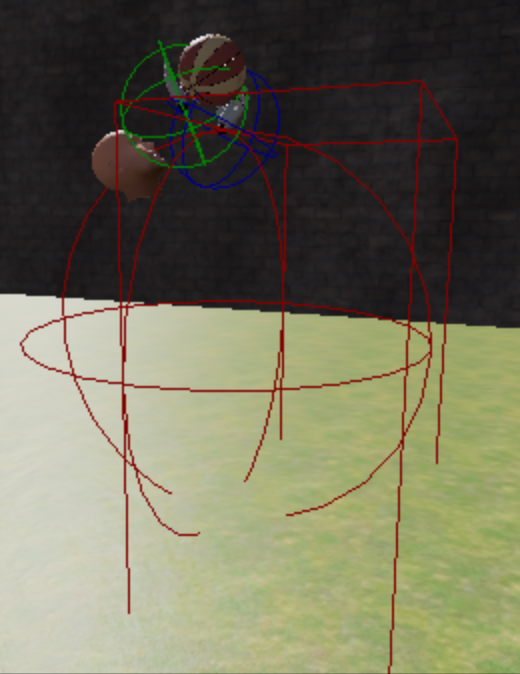
\includegraphics[width=1.0\linewidth]{PlaybackActor.png}
\caption{Beispiel einer Wiedergabe mit den drei Hüllkörpern. Die Kugeln um die Hände sind hier blau und grün dargestellt. Die Halbkugel für den Körper wird aus dem Schnitt des roten Quaders und der roten Kugel gebildet, da die Unreal Engine keine Halbkugeln als Hüllkörper anbietet.}
\label{fig:playback-actor}
\end{figure}
Bei der Wiedergabe werden das HMD und die Controller durch Modelle von Kopf und Händen dargestellt. Sie besitzen Hüllkörper, mit denen die Gegenstände in der Nähe der Hände bzw. des Körpers ermittelt werden. Sie repräsentieren somit wie in \cite{scene-grok} die \textit{aktiven Objekte}. Wir verwenden hierzu ebenfalls Kugeln für die Hände und eine Halbkugel, die vom Kopf senkrecht nach unten verläuft für den Bereich vor dem Körper (siehe Abbildung \ref{fig:playback-actor}. Hier ist die Tasse in der rechten Hand ein aktives Objekt). Die Radien sind über die Einstellungen anpassbar. Zudem können bei der Wiedergabe zugleich die Merkmalsvektoren mit berechnet werden.

\subsection{Merkmalsvektoren erstellen}
\label{subsec:merkmalsvektoren-erstellen}
Welche Merkmale verwendet werden sollen, wird im Quelltext angegeben. Die Unreal Engine bietet mit den sogenannten Blueprints eine graphenbasierte Alternative zur C++-Programmierung an. Die von uns erstellte Blueprintfunktion \glqq{}logFeatures\grqq{} hat als Inputparameter die Kalibrierungsdaten, alle Informationen zu Kopf und Händen und eine Liste mit den Featurevektoren, an den jeder neu berechnete Vektor angehangen wird. Ein kurzes Beispiel ist in Abbildung \ref{fig:log-features} zu sehen. Dort werden als Merkmale die Höhe des Kopfes und dessen Abstände zu den beiden Händen berechnet. Dafür wird zunächst die Raumposition (\glqq{}GetWorldLocation\grqq{}) der Hände und des Kopfs bzw. deren Hauptkomponenten (\glqq{}Default Scene Root\grqq{}) ausgelesen. Das erste Merkmal ist die Z-Komponente, also die Höhe des HMDs über dem Boden, dividiert durch die zuvor in der Kalibrierung gemessene Höhe des Nutzers. Die Merkmale zwei und drei ergeben sich aus dem euklidischen Abstand zwischen dem Kopf und den Händen. Auch hier wird zur Normierung durch die zuvor gemessene Armlänge geteilt. Die Merkmale werden zusammengefasst und an die Liste mit den vorherigen Merkmalsvektoren angehangen. Die von uns verwendeten Merkmale werden im Abschnitt \ref{subsec:auswahl-der-feature-vektoren} genauer beschrieben.
\begin{figure}[hbtp]
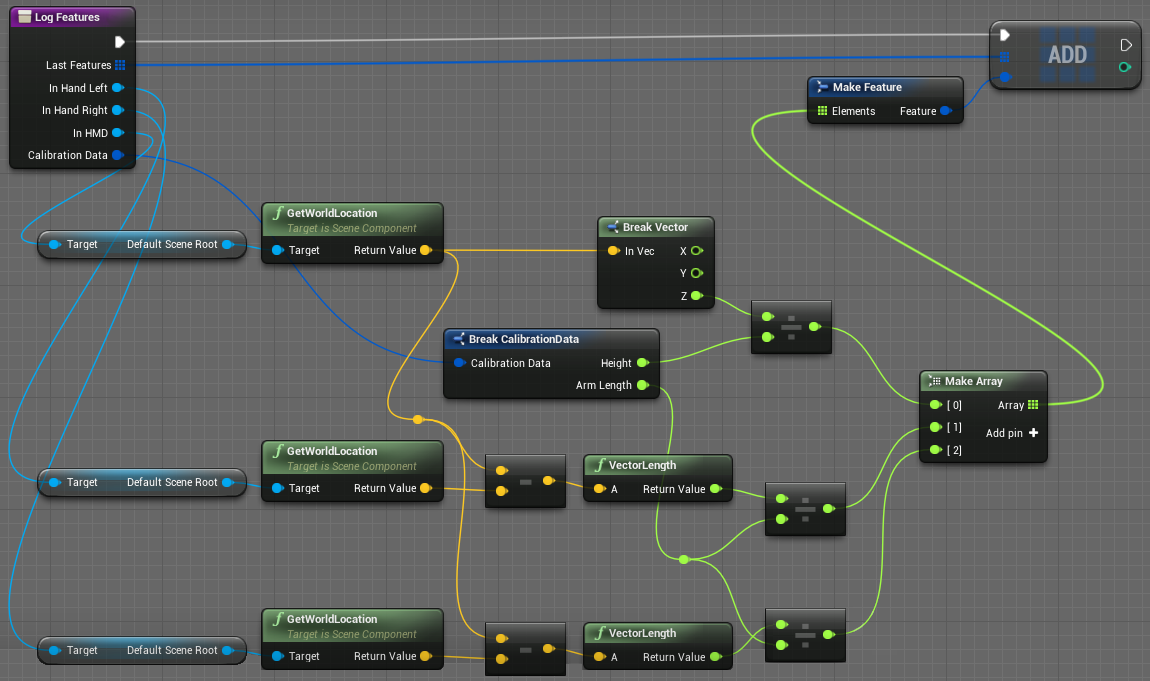
\includegraphics[width=1.0\linewidth]{LogFeatures.png}
\caption{Merkmalsvektoren im Blueprint erstellen}
\label{fig:log-features}
\end{figure}

\subsection{Trainings- und Testdaten erstellen}
\label{subsec:trainings-und-testdaten-erstellen}
Nachdem die Featurevektoren herausgeschrieben wurden, kann das Trainingsmodell erstellt werden. Hierfür verwenden wir die Support-Vector-Machine libsvm (siehe Abschnitt \ref{subsec:libsvm}). Um das Modell zu generieren, benötigt die SVM Trainings- und Testdaten, die wir aus den aufgenommenen Merkmalsvektoren erstellen. Diese liegen in dem Unterordner \glqq{}Features\grqq{} des Aufnahmeverzeichnisses. Zu jeder Aufnahme existiert eine entsprechende Datei mit den Featurevektoren. Da die libsvm nur Zahlen als Label der Aktionen verwendet, befindet sich dort zudem eine Datei, die jeder Gruppe von Aktionen einen Index zuordnet. Mit einem Skript können die Hälfte der Aufnahmen jeder Gruppe in einer Testdatei und die andere Hälfte in einer Trainingsdatei zusammengefügt werden. Aus den Trainingsdaten erstellt die libsvm im Anschluss ein Trainingsmodell, auf dessen Grundlage die Klassifizierung der Test- bzw. Livedaten erfolgt.

\subsection{Live Klassifizierung}
Bei der Live Klassifizierung werden vom Benutzer Aktionen ausgeführt und daraus in Echtzeit die Featurevektoren bestimmt. Zu diesem Zweck haben wir die libsvm über C++ an das Framework angebunden ist. Zu Beginn wird das zuvor generierte Klassifizierungsmodell von der SVM geladen. Während der Live Klassifizierung werden dann, wie zuvor beim Erstellen der Trainingsdaten, in regelmäßigen Abständen die Merkmalsvektoren für den aktuellen Zeitpunkt berechnet. Die SVM wertet jeden Featurevektor auf der Grundlage des trainierten Modells aus und prognostiziert die Art der dargestellten Aktion. Wir stabilisieren das Ergebnis im Anschluss noch, indem immer die Prognose ausgeben wird, die unter den letzten 10 Klassifizierungen am häufigsten aufgetreten ist. 


%%%%%%%%%%%%%%%%%%%%%%%%%%%%%%%%%%%%%%%%%%%%%%%%%%%%%%%%%%%%

\section{Support Vector Machine SVM \tiny{(Dominik Blitsch)}}
\label{sec:support-vector-machine-svm}

\subsection{Einführung}
\label{subsec:einfuehrung}
Eine Support Vector Machine führt eine Klassifikation von Objekten anhand von bereits klassifizierten Objekten aus. Die Objekte werden als n-dimensionale Vektoren $v$ im Objektraum $X \subseteq \mathbb{R}^{n} $ dargestellt, bei denen je ein Wert ein bestimmtes Merkmal (hier Feature) des Objektes darstellt. Zur Klassifizierung wird der Objektraum durch Hyperebenen so geteilt, dass jede Klasse von den anderen getrennt ist. Das heißt es erfolgt eine Zuordnung des Objektraumes $X$ zum Ergebnisraum $Y = {1,...,m} \subseteq \mathbb{R}$, der alle Klassen beinhaltet. Zur Berechnung dieser Hyperebenen dienen die Trainingsdaten $T =((x_{1},y_{1}),...,(x_{l},y_{l})) \subseteq (X \times Y)^{l}$, die der SVM übergeben werden. Somit besteht jedes Trainingsset aus einem Objekt $x_{i} \in X$ und der dazugehörigen Klasse $y_{i} \in Y$. Die Hyperebenen werden so gewählt, dass der mögliche Unterschied innerhalb einer Klasse möglichst groß ist. Dies wird dadurch realisiert, dass die Abstände der Vektoren, die der Hyperebene am Nächsten liegen maximiert werden (Maximum Margin). Diese der Hyperebene am nächsten gelegenen Vektoren werden \glqq{}Support-Vectors\grqq{} genannt, da durch diese die optimale Hyperebene \glqq{}stabilisiert\grqq{} wird. Jedoch lassen sich nicht alle Datenpunkte durch Hyperebenen trennen, da es Ausreißer geben kann und Klassen sich teilweise sogar überschneiden. Um diese Daten zu klassifizieren, bedient sich die SVM des Kerneltricks. \cite{laechele-svm}

\subsection{Lineare Klassifikation}
\label{subsec:lineare-klassifikation}
Die einfachste Art der linearen Klassifikation ist die binäre Klassifikation. Hierbei werden die Vektoren mit Hilfe der Funktion $ f: X \subseteq \mathbb{R} \rightarrow \mathbb{R} $ der positiven $ (f(x)>0) $ oder negativen $ (f(x)<0) $ Klasse zugeordnet. Die trennende Hyperebene lässt sich durch einen Normalenvektor $\vec{\omega} \in X$ und ein Offset $b$ beschreiben.
Damit gilt:\[ f(\vec{x})=\left\langle \vec{\omega} \cdot \vec{x} \right\rangle\ + b = \sum\nolimits_{i=1}^n \omega_{i} x_{i} + b \]
Mit der Entscheidungsfunktion $h : \mathbb{R} \rightarrow \{-1,1\}$:
\[ h(x) = sign(f(x)) = sign (\sum\nolimits_{i=1}^n \omega_{i} x_{i} + b)\]
Eingabevektoren, die sich auf diese Weise trennen lassen, werden linear separabel genannt. Ein Beispiel für linear separierbare Daten ist in Abbildung \ref{fig:LinSeparabel} zu sehen. Hier kann man gut erkennen, dass sich auf einer Seite der Hyperebene (im $\mathbb{R}^2$ eine Gerade) auch nur eine Klasse von Daten (rot oder grün) befindet.

\begin{figure}[hbtp]
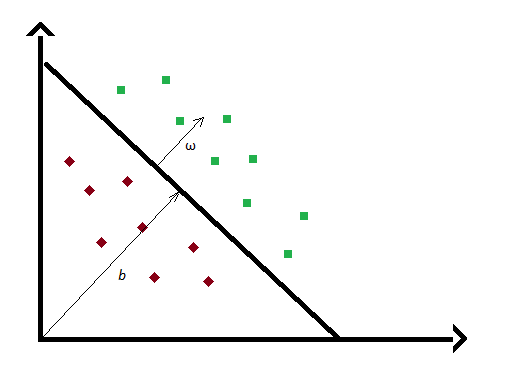
\includegraphics[width=0.7\linewidth]{LinSeparabel.png}
\centering
\caption{Beispiel für linear separierbare Eingabevektoren. Die Vektoren werden mit Hilfe von h(x) in zwei Klassen überhalb (positiv bzw. grün) und unterhalb (negativ bzw. rot) der Geraden eingeteilt. $\omega$ bestimmt hierbei die Steigung der Geraden, während $b$ sie parallel verschiebt.}
\label{fig:LinSeparabel}
\end{figure}\ \\
Eine lineare Klassifikation, deren Ausgaberaum mehr als 2-dimensional ist $(Y = \{1,...,n\})$, lässt sich durch $n$ binäre Klassifikationen simulieren. Hierbei wird für jede Klasse eine binäre Klassifikation durchgeführt und dann die Eingabe $x$ der Klasse zugeordnet, deren Hyperebene am weitesten entfernt ist.\\ \\
Um die optimale Hyperebene zu einer binären Klassifikation mittels \glqq{}Maximum Margin Classificator\grqq{} zu finden, benötigen wir einige Definitionen: \\
 Der Abstand $\gamma_{i}$ (bzw. Margin) zwischen einem Beispiel $(x_{i},y_{i})$ und einer Hyperebene ist gegeben durch:
\[ \gamma_{i} = y_{i}(\langle \omega \cdot x_{i} \rangle + b )\]
Des weiteren ist der Abstand einer Hyperebene $\gamma$ zu mehreren Trainingsdaten das Minimum über alle $\gamma_{i}$.
\[\gamma = min_{i\leq l} \gamma_{i}\]
Die optimale Hyperebene ist nun diejenige, deren Margin zu dem Trainingsset maximal ist. Hierzu werden zwei zu der Hyperebene parallele Ebenen mit dem Abstand $\gamma$ definiert. Die Vektoren, die $\gamma$ beschränken, deren Abstand zur Hyperebene minimal ist, sind die \glqq{}Support-Vectors\grqq{}. Damit lässt sich der $\gamma$ über den Normalenvektor der Hyperebene berechnen:
\[\gamma = \frac{1}{\lVert \omega \rVert_{2}} \]
Damit ergibt sich folgendes Optimierungsproblem:\\

\qquad minimiere$_{\omega,b}$ \hfill $\langle \omega \cdot \omega \rangle,$ \\

\qquad in Abhängigkeit von \hfill $\gamma_{i}(\langle \omega \cdot x_{i} \rangle + b) \geq 1 $ \\\\
Mit Hilfe der Formel von Lagrange lässt sich dieses Problem durch die Lagrange-Multiplikatoren $\alpha_{i}$ in primärer Form schreiben:
\[ L(\omega,b,\alpha) = \frac{1}{2} \langle \omega \cdot \omega \rangle -  \sum\nolimits_{i=1}^l \alpha_{i} \lbrack \gamma_{i} (\langle \omega \cdot x_{i} \rangle + b) -1 \rbrack\]
Durch Ableiten nach $\omega$ und $b$ und anschließender Resubstitution in die primäre Form ergibt sich das Optimierungsproblem in dualer Form: \\\\

\qquad maximiere \hfill $L(\omega,b,\alpha) = \sum\nolimits_{i=1}^l \alpha_{i} - \frac{1}{2} \sum\nolimits_{j=1}^l \gamma_{i} \gamma_{j} \alpha_{i} \alpha_{j} \langle x_{i} \cdot x_{y} \rangle$ \\\\

\qquad in Abhängigkeit von \hfill $\sum\nolimits_{i=1}^l \gamma_{i} \alpha_{i} = 0$\\

\hfill $ \alpha_{i} \geq 0: i = 1,...,l$\\
Dieses Problem kann iterativ gelöst werden.\cite{laechele-svm}

\subsection{Kerneltrick}
\label{subsec:kernel-trick}
Wie bereits angesprochen lassen sich nicht alle Klassen im Objektraum durch Hyperebenen trennen. Häufig sind die Klassen nicht linear separabel und können somit nicht durch den \glqq{}Maximal Margin Classifier\grqq{} getrennt werden. Um Datenpunkte dieser Klassen dennoch richtig zuordnen zu können, bedient man sich des Kerneltricks. Hierbei wird der Objektraum $X$ durch die Funktion $\phi$ auf einen höherdimensionalen Merkmalsraum $F$ abgebildet:
\[\phi : X \subseteq \mathbb{R}^l \rightarrow F \subseteq \mathbb{R}^k\ mit\ l<k \]
In dem Merkmalsraum $F$ kann nun die SVM eine Hyperebene finden und somit können die Datenpunkte klassifiziert werden. In Abbildung \ref{fig:Objektraum-Merkmalsraum} sind Datenpunkte zweier Klassen (rot und grün) zu erkennen, die durch die Funktion $\phi$ in den Merkmalsraum übertragen werden und somit linear separabel werden.\\
\begin{figure}[hbtp]
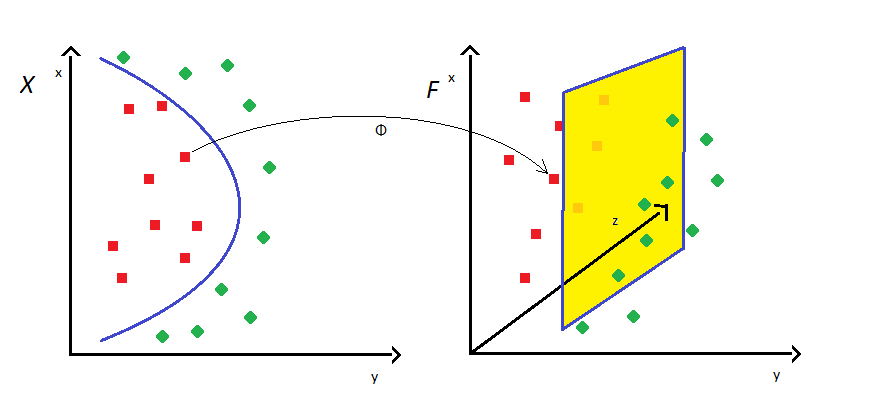
\includegraphics[width=1.0\linewidth]{ObjektZuMerkmalsRaum.png}
\caption{Die nicht linear separablen Datenpunkte im Objektraum $X \subseteq \mathbb{R}^2$ (linkes Koordinatensystem) werden durch die Funktion $\phi$ in einen Merkmalsraum $F\subseteq \mathbb{R}^3$ (rechtes Koordinatensystem) abgebildet und können dort durch eine Ebene getrennt werden.}
\label{fig:Objektraum-Merkmalsraum}
\end{figure}\\
Da die Vektoren im Optimierungsproblem nur als Skalarprodukte auftreten, muss man den Merkmalsraum nicht kennen. Es reicht, wenn man die Skalarprodukte im Objektraum durch eine Funktion $K$ berechnen kann:
\[K(x,y) = \langle \phi(x) \cdot \phi(y) \rangle,\ x,y \in X\]
Eine solche Abbildung nennt man Kernel. Diese lässt sich für das Skalarprodukt in das Optimierungsproblem einsetzen, sodass man nun die Datenpunkte klassifizieren kann.\cite{laechele-svm,sayad-svm}


\subsection{LIBSVM}
\label{subsec:libsvm}
Die Featurevektoren werden wie in den Abschnitten \ref{subsec:merkmalsvektoren-erstellen} und \ref{subsec:trainings-und-testdaten-erstellen} beschrieben mit der Unreal Engine berechnet und jeder Klasse eine eindeutige Zahl zugewiesen. Danach wird ein Trainingsset $(x_{i}:y_{i}), x_{i} = (x_{i1},x_{i2},...,x_{il}) \in X, y_{i} \in Y$ LIBSVM in einer Textdatei folgendermaßen übergeben:
\begin{tabbing}
\qquad \= $... $\\
\>$ y_{i}\ \ \ \ 1:x_{i1}\ \ \ \ 2:x_{i2}\ \ \ \ ...\ l-1:x_{il-1}\ \ \ \ l:x_{il} $\\
\>$ y_{i+1}\ 1:x_{i+11}\ 2:x_{i+12}\ ...\ l-1:x_{i+1l-1}\ l:x_{i+1l} $\\
\>$ ... $\\
\end{tabbing}
Als Implementierung der SVM haben wir die C++ bzw. Java-Bibliothek LIBSVM genutzt. Der Vorteil hierbei ist, dass diese frei verfügbar ist und gewisse Funktionen bereits enthält. So kann ein Datensatz aufgeteilt werden, um mit dem ersten Teil zu trainieren und mit dem zweiten Teil zu testen, wie gut die durch das Training erstellte Zuordnung ist (Cross-Validation). Dabei wird der Prozentsatz der richtig klassifizierten Datensätze ausgeben, sodass man sehr schnell und einfach einen Vergleich der ausgewählten Features durchführen kann. 

\subsection{Auswahl der Featurevektoren}
\label{subsec:auswahl-der-feature-vektoren}
Die richtige Anzahl und Auswahl der Merkmale im Featurevektor ist essenziell für eine gute Klassifizierung, da die Vektoren unterschiedlicher Klassen auch möglichst unterschiedlich sein müssen, damit die SVM trennende Hyperebenen findet. Deshalb haben wir uns zunächst für einen Merkmalsraum in der 10. Dimension entschieden, um möglichst viele Unterschieden zwischen Klassen erkennen zu können. Unsere Features hierbei waren:
\begin{itemize}
    \item Kopfhöhe \ \ \quad\qquad\qquad\qquad\qquad\qquad\qquad\qquad$h \in \mathbb{R}$
    \item Blickrichtung \qquad\qquad\qquad\qquad\qquad\qquad\qquad$b \in \mathbb{R}^3$
    \item Richtungsvektor von Kopf zu rechter Hand \quad $r \in \mathbb{R}^3$    
    \item Richtungsvektor von Kopf zu linker Hand \ \ \quad $l \in \mathbb{R}^3$
\end{itemize}
\begin{figure}[hbtp]
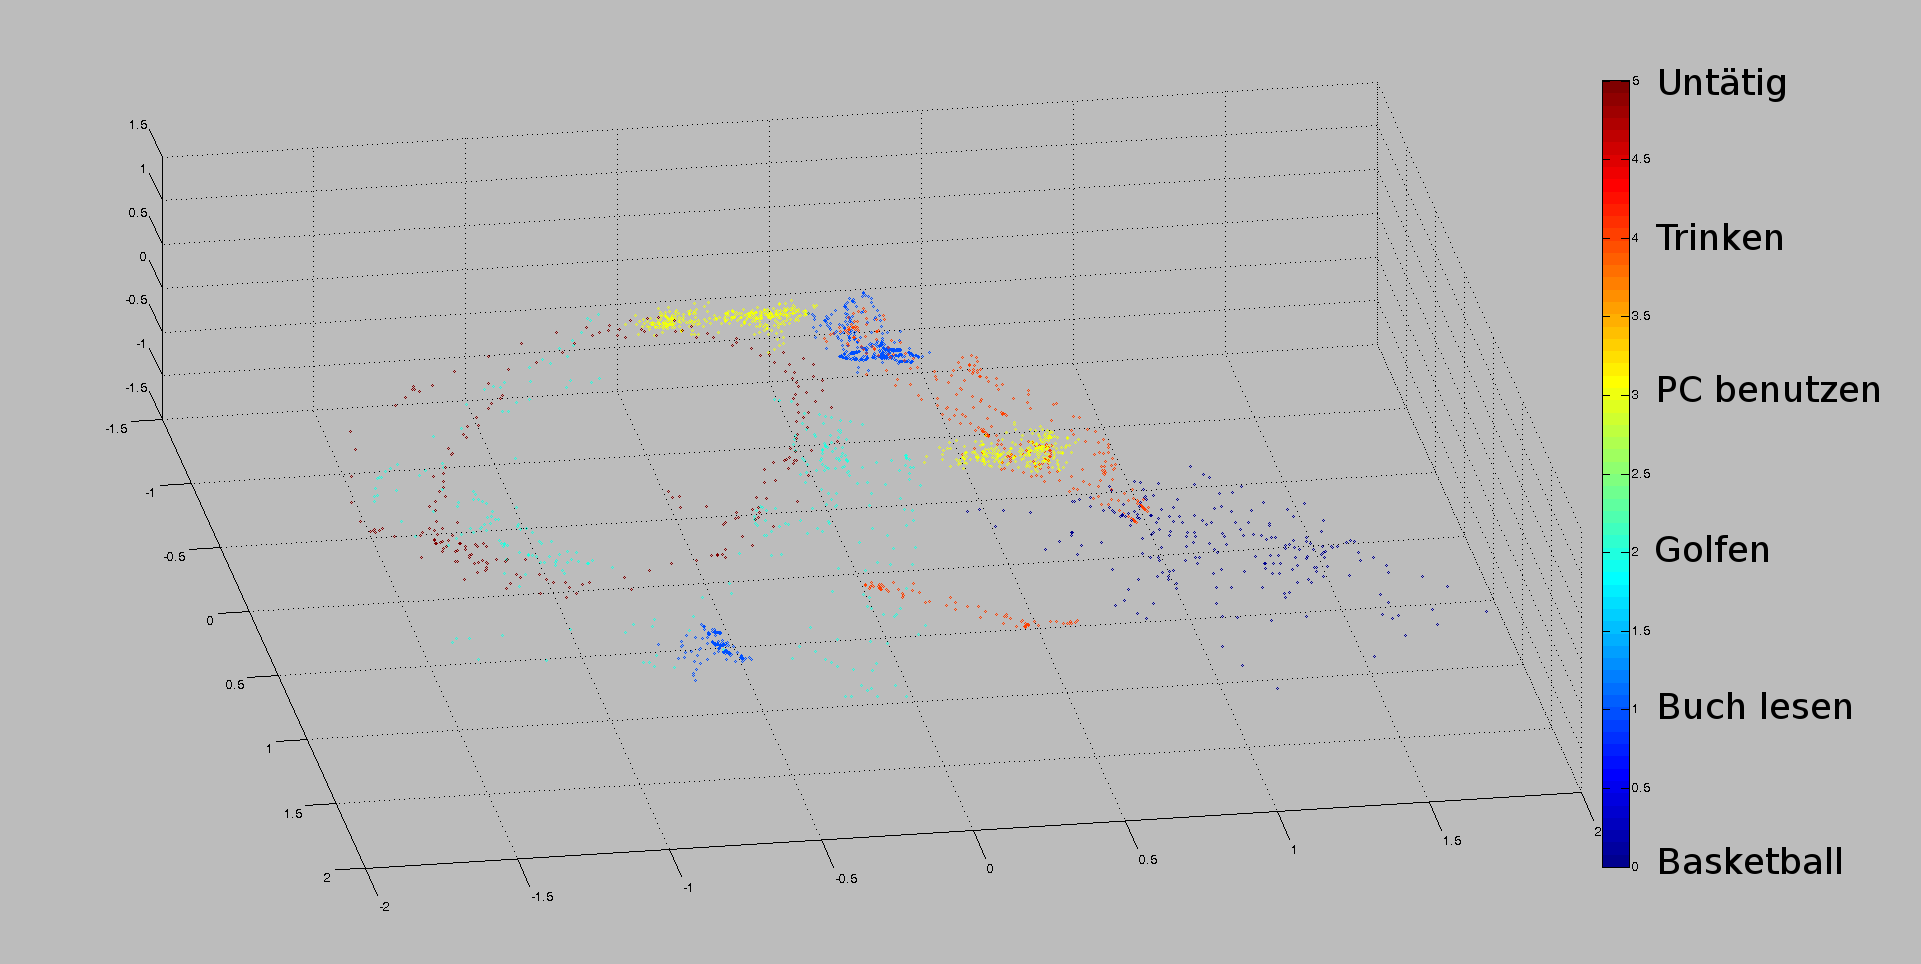
\includegraphics[width=1.0\linewidth]{OldFeatures.png}
\caption{Hier sind die Datensätze der ersten Features ($h$, $b$, $r$, $l$) zu sehen. Um den 10-Dimensionalen Featureraum beobachtbar zu machen, wurde er per Multi-Dimensional-Scaling in den $\mathbb{R}^3$ überführt.}
\label{fig:Old-Features}
\end{figure}
Wie in Abbildung \ref{fig:Old-Features} zu sehen, sind die Vektoren einer Klasse häufig nicht geclustert, sondern über große Bereiche verteilt. So sieht man zum Beispiel, dass die Daten der Aktion \glqq{}PC benutzen\grqq{} in zwei Bereichen auftauchen. Diese Aktion wurde von uns in zwei verschiedenen und unterschiedlich orientierten Szenen aufgenommen. Dadurch, dass wir die Blickrichtung $b$ als Feature genommen haben, sind die Vektoren je nach Szene sehr unterschiedlich, obwohl jeweils die gleiche Aktion ausgeführt wurde. Dies sorgt dafür, dass die einzelnen Aktionen nicht gut voneinander getrennt werden können und somit eine passende Klassifikation fehlschlägt. Daran erkennt man sehr gut, dass die Blickrichtung als Feature nicht geeignet ist. Auch die Vektoren zu den Händen $l,r$ sind richtungsabhängig und daher als Merkmale ebenfalls nicht gut geeignet.\\
Dieser Featurevektor ist also nicht gut besonders ideal um Aktionen zu klassifizieren. Das zeigt sich auch in der Trainings- und Testfunktion der LIBSVM. Dort war die Klassifizierung der Testdaten nach dem Training nur bei etwas über 40\%. Bei 6 Aktionen ist das zwar deutlich über einer randomisierten Klassifikation, aber für den betriebenen Aufwand deutlich zu wenig.\\
Deshalb haben wir uns dann entschlossen die Features etwas zu reduzieren, sodass diese innerhalb einer Klasse möglichst ähnlich bleiben und nicht von dem verwendeten Szenen oder der Richtung abhängen. Außerdem haben wir die in \cite{scene-grok} definierten Bounding Boxes um den Körper genutzt, um Informationen über möglicherweise verwendete Szenenelemente zu bekommen. Dadurch ergaben sich folgende Merkmale:
\begin{itemize}
    \item Höhe des Kopfes $h$
    \item kleinere Entfernung vom Kopf zur Hand $min(\lVert l \rVert,\lVert r \rVert)$
    \item größere Entfernung vom Kopf zur Hand $max(\lVert l \rVert,\lVert r \rVert)$
    \item Gewicht des Objektes mit dem geringsten Abstand zu einer Hand $g$
\end{itemize}
Um eine Unabhängigkeit bei der Ausführung einer Aktion mit rechter oder linker Hand zu gewährleisten, haben wir die Entfernungen zu den Händen als größere und kleinere Entfernung in den Featurevektor eingetragen. Somit haben wir einen Featurevektor der Aktionen gut unterscheidet, auch wenn diese in unterschiedlichen Szenen oder in unterschiedlichen Richtungen ausgeführt werden.

\subsection{Qualität der Featurevektoren}
\label{subsec:qualitaet-der-feature-vektoren}
Als ersten Test der neuen Featurevektoren haben wir die Testfunktion der LIBSVM genutzt. Hierbei bekamen wir eine richtige Klassifizierung in 98\% der Testdaten. Eine so gute Klassifizierung kann häufig auch dem so genannten \glqq{}Overfitting\grqq{} geschuldet sein. Das bedeutet, dass die Hyperebenen die Datenpunkte sehr eng umschließen und somit sehr ähnliche Featurevektoren sehr gut erkannt werden, aber sobald eine leichte Abweichung des Standardfalls auftritt, wird der Vektor der falschen Klasse zugeordnet. Um dies auszuschließen, haben wir mehrere Live-Klassifizierungs-Tests gemacht, in denen wir die Aktionen mit sehr unterschiedlichen Bewegungsabläufen wiederholt haben. Auch hier wurde unsere Bewegung sehr gut klassifiziert, sodass Overfitting ausgeschlossen werden konnte.
\begin{figure}[hbtp]
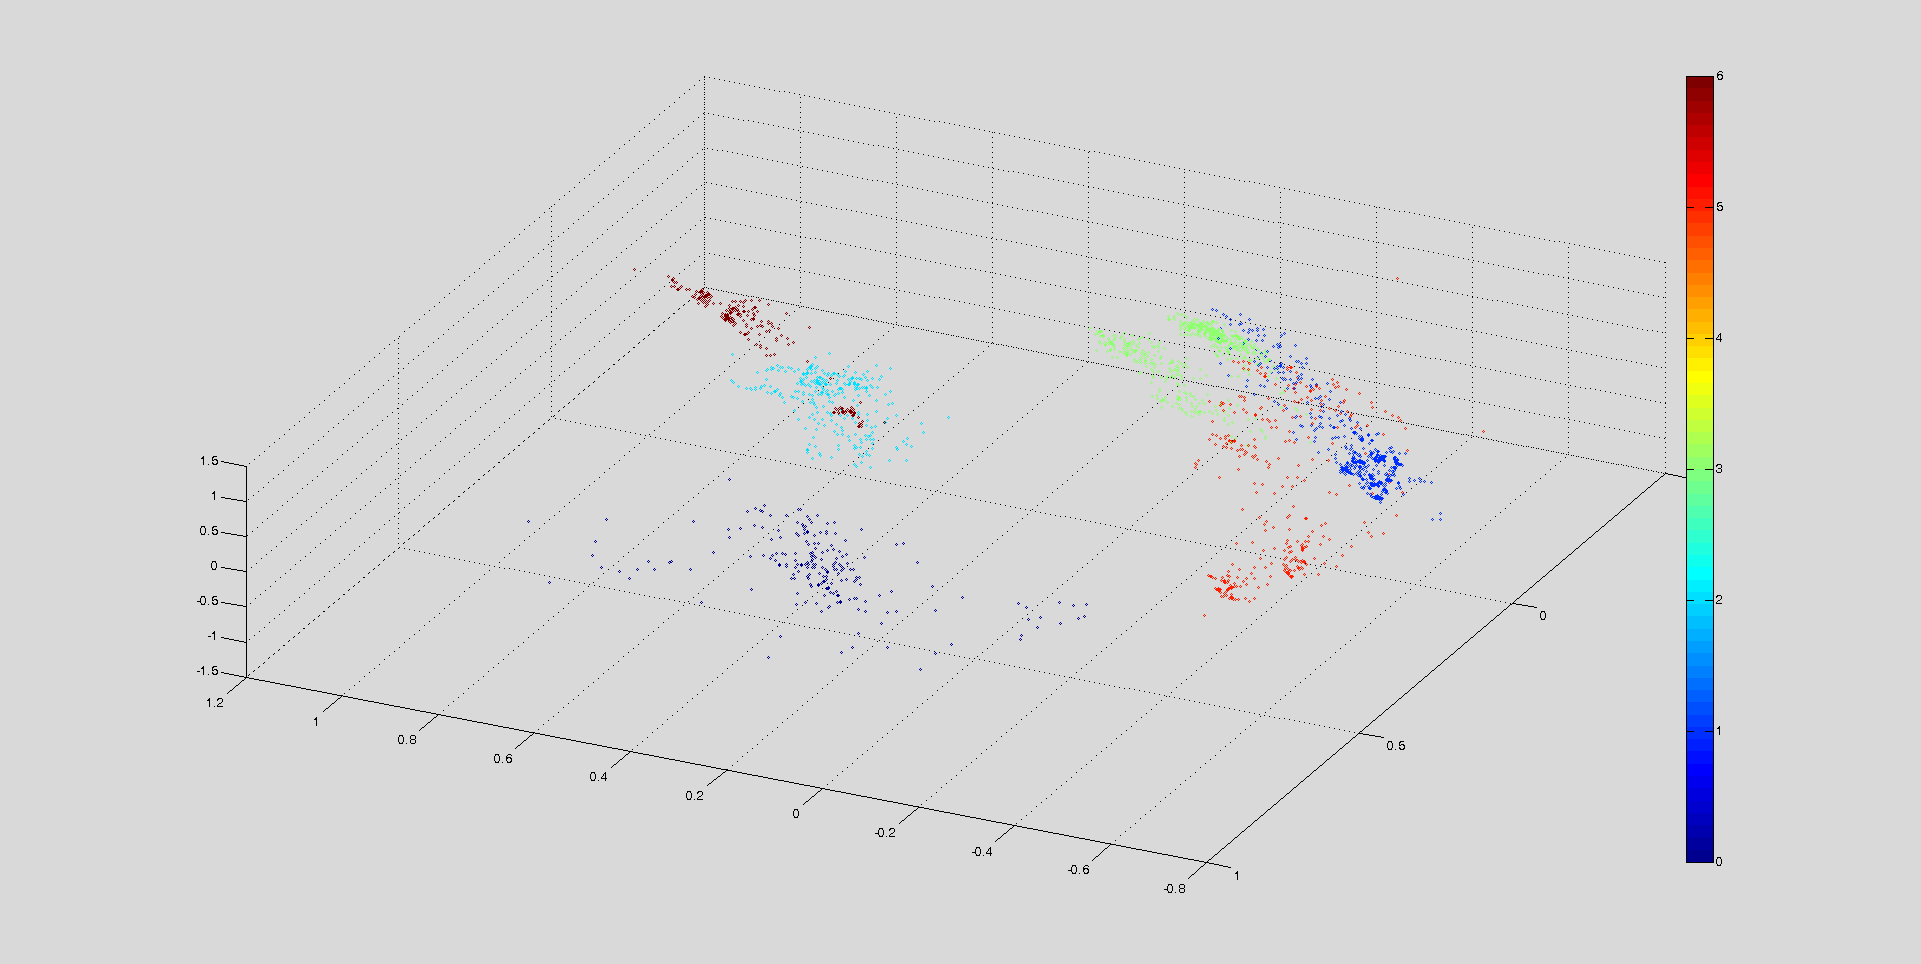
\includegraphics[width=1.0\linewidth]{NewFeatures.png}
\caption{Hier sind die Datensätze der finalen Features zu sehen. Auch hier wurde der Featureraum mittels Multi-Dimensional-Scaling in den $\mathbb{R}^3$ überführt.}
\label{fig:New-Features}
\end{figure}
Wie in Abbildung \ref{fig:New-Features} zu sehen, sind die Datenpunkte einer Aktion jeweils in einem Bereich geclustert. Dadurch kann die SVM sehr leicht trennende Hyperebenen finden, sodass eine Aktion richtig klassifiziert wird.

\subsection{Gewicht ohne Virtual Reality}
\label{subsec:gewicht-ohne-virtual-reality}
Um Aktionen ohne Virtual Reality durchzuführen, müssen sowohl die Datenaufnahme als auch die Featurevektoren sinnvoll überführt werden. Die Datenaufnahme kann durch verschiedene Scansysteme ausgeführt werden, sodass Bewegungen und Aktionen in für Computer verständliche Daten verarbeitet werden. Somit können Abstände sehr gut eingescannt werden. Um allerdings das Gewicht der Objekte zu erfassen, müsste jedes verwendete Objekt gewogen werden. Da dies im Allgemeinen nicht praktikabel ist, kann das Gewicht nicht als Feature zur Klassifizierung genutzt werden. Allerdings können andere Größen von Objekten besser erfasst in somit verwendet werden. Zum Beispiel kann durch einen Scanner das Volumen oder die Oberfläche eines Objektes gut eingelesen werden. Das kann selbst dann funktionieren, wenn das Objekt nicht alleine in einem Raum ist. Also können auch ohne Virtual Reality Eigenschaften von Objekten für die Klassifizierung von Aktionen genutzt werden. Das diese Technik zu einer sehr guten Qualität der Klassifikation führt, zeigt die zuverlässige Vorhersage während der Live-Klassifizierung.

%%%%%%%%%%%%%%%%%%%%%%%%%%%%%%%%%%%%%%%%%%%%%%%%%%%%%%%%%%%%

\section{Limitationen \tiny{(Mohammad Vosoughi)}}
\label{sec:limitation}

Wir konnten den Aufwand Aktionen in realen Szenen aufzunehmen durch die Verwendung von virtuellen Szenen und dem VR-System HTC Vive stark reduzieren. Allerdings treten dadurch auch neue Schwierigkeiten auf. Mit der HTC Vive lassen sich nur die Positionen und Orientierungen der Hände und des Kopfs verfolgen. Bei vielen Aktionen ist jedoch auch die Interaktion von anderen Körperteilen mit der Umgebung entscheidend. Zum Beispiel ist es für die Aktion \glqq{}Fußball spielen\grqq{} entscheidend, dass sich ein Ball in der Nähe eines Fußes befindet. Um solche Aktionen genau zu beschreiben, ist es dann notwendig, mehrere Tracker zu verwenden. In Abbildung \ref{fig:Human-Body} sind die relevanten Positionen für solche Tracker markiert. Ein interessanter Ansatz mit weniger Trackern auszukommen wird in \cite{body-reconstruction} beschrieben. Dort wird eine Methode vorgestellt, mit der sich die Körperhaltung in Echtzeit nur aus den Positionen und Orientierungen von Kopf und Händen rekonstruieren lässt.\newline
\begin{figure}[hbtp]
\centering
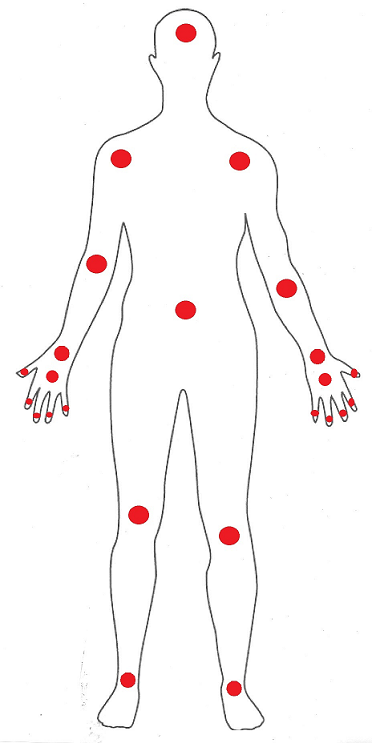
\includegraphics[width=0.2\linewidth]{human_body1.png}
\caption{Menschlicher Körper. Die roten Punkte beschreiben die annehmbaren Positionen der Tracker}
\label{fig:Human-Body}
\end{figure}

Wie im Abschnitt \ref{subsec:auswahl-der-feature-vektoren} beschrieben, verwenden wir neben der Masse des nächsten Gegenstandes die Kopfhöhe und den minimalen und maximalen Abstand der Hand zum Kopf. Diese werden in unserem Fall 5 mal in der Sekunde aufgenommen und beschreiben so die dargestellte Pose. Eine Aktion ist eine geordnete Abfolge dieser Merkmale. Wir haben aber die Reihenfolge der Merkmale beim Trainieren unserer SVM nicht berücksichtigt. Die Merkmalsvektoren sind daher auch bei verschiedenen Aktionen oftmals recht ähnlich. In Abbildung \ref{fig:Merkmalvektoren-Diagramm} ist das gut zu erkennen. Hier liegen die Merkmale der Aktionen Basketball (dunkelblau) und Trinken (dunkelrot) nah zueinander, da sowohl beim Basketball als auch beim Trinken eine Nickbewegung des Kopfes ausgeführt wird.\newline
\begin{figure}[hbtp]
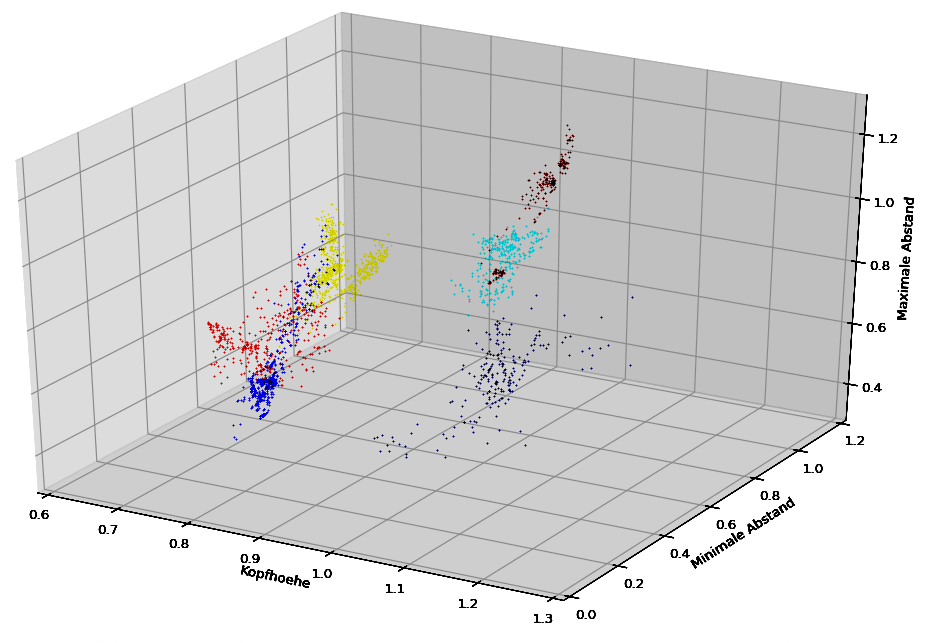
\includegraphics[width=1.0\linewidth]{moplot.png}
\caption{Featurevektor-Diagramm. Rechts sind die Aktionen und deren Farben im Diagramm aufgelistet. Von unten nach oben: 1 - Basketball spielen, 2 - Buch lesen, 3 - Golfen, 4 - PC benutzen, und 5 - trinken }
\label{fig:Merkmalvektoren-Diagramm}
\end{figure}
Aufgrund der Ähnlichkeit fällt in diesen Fällen die Masse des nächsten Gegenstandes stärker ins Gewicht. Haben dann die Szenenobjekte ähnliche Massen, wie die Getränkeflasche und der Basketball, kann das zu Fehlklassifizierungen führen. Wird zum Beispiel im Stehen aus einer Flasche getrunken, so kann die Aktion fälschlicherweise als \glqq{}Basketball spielen\grqq{} klassifiziert werden. 

\section{Diskussion und Ausblick \tiny{(Mohammad Vosoughi)}}
\label{diskussion-ausblick}
Wir haben eine Methode zur Erforschung von Aktionen vom Menschen in virtueller Realität vorgestellt. Diese Methode bildet Merkmalsvektoren aus der Pose eines Menschen und den Eigenschaften der Gegenstände aus der Szene und verwendet dabei eine SVM als Klassifizierer. Um die Pose der durchführenden Person darzustellen, wurden die Kopfhöhe und die Abstände von den Händen zum Kopf genutzt und unter Berücksichtigung der Körpermaße des Nutzers kalibriert. 


\subsection{Maschinelles Lernen kombiniert mit Automaten}
Da wir die Reihenfolge der Merkmalvektoren in Relation mit den Aktionen nicht berücksichtigen, bietet es sich an, die Pose in Zustände zu unterteilen und die Reihenfolge der verschiedenen Zustände und die jeweilige Interaktion mit den Gegenständen als eine Aktion zu betrachten. Damit sollte die verwendete SVM in der Lage sein, nicht lineare multidimensionale Funktionen voneinander zu unterscheiden.

\subsection{Körperrekonstruktion}
Für genauere Aktionserkennungen sollte die Pose des Nutzers besser rekonstruiert werden. Hierfür bietet es sich an, mehr Körperteile zu tracken oder die in \cite{body-reconstruction} beschriebene Methode zur Echtzeit-Körperrekonstruktion zu implementieren.



%%%%%%%%%%%%%%%%%%%%%%%%%%%%%%%%%%%%%%%%%%%%%%%%%%%%%%%%%%%%

